%!TEX root = ../thesis.tex
%*******************************************************************************
%******************************* Instructions **********************************
%*******************************************************************************

\ifpdf
    \graphicspath{{Instructions/Figs/Raster/}{Instructions/Figs/PDF/}{Instructions/Figs/}}
\else
    \graphicspath{{Instructions/Figs/Vector/}{Instructions/Figs/}}
\else
    \graphicspath{{Instructions/Figs/Regular/}{Instructions/Regular/}}    
\fi

\thispagestyle{empty}
 \newpage
 \newpage
\begin{center}
\section*{Instruc\c{t}iuni de redactare pentru doctoranzi}
\vspace{-0.5cm}
(\textcolor{red}{acest text nu face parte din tez\u{a}})
\end{center}

\thispagestyle{empty}
\subsection*{Instruc\c{t}iuni de formatare generale}
\begin{itemize}
  \item Teza se redacteaz\u{a} \^{i}n format A4, la 1,15 r\^{a}nduri, cu caractere Times New Roman de 12pt. \c{s}i diacritice. Tip\u{a}rirea se face pe ambele fe\c{t}e ale foii A4.
  \item Marginile textului sunt la 1,5$''$ (3,5 cm) st\^{a}nga \c{s}i 1$''$ (2,5 cm) dreapta, sus \c{s}i jos. Num\u{a}rul paginii se insereaz\u{a} jos, central, la cel pu\c{t}in 0,75$''$ (2 cm) de marginea de jos a paginii. Coperta interioar\u{a} nu se pagineaz\u{a}.
  \item Paginile de: Mul\c{t}tumiri, Cuprins, Lista tabelelor, Lista figurilor şi Lista abrevierilor se pagineaz\u{a} cu cifre romane mici: i, ii, iii, etc.
  \item Capitolele, bibliografia \c{s}i anexele se pagineaz\u{a} cu cifre arabe. Excep\c{t}ie face prima pagin\u{a} a fiec\u{a}rui capitol, pe care num\u{a}rul paginii nu trebuie să apar\u{a}.
  \item Paginile pare ale capitolelor au în antet titlul tezei scris cu caractere Times New Roman de 10pt. La nevoie, titlul trebuie prescurtat astfel \^{i}nc\^{a}t s\u{a} \^{i}ncap\u{a} pe un singur r\^{a}nd.
  \item Paginile impare ale capitolelor au \^{i}n antet titlul capitolului scris cu caractere Times New Roman de 10pt. Excep\c{t}ie face prima pagin\u{a} a fiec\u{a}rui capitol.
  \item Teza cuprinde, \^{i}n ordine, urm\u{a}toarele sec\c{t}iuni/informa\c{t}ii:
  \begin{itemize}
  \item Coperta interioar\u{a} (pagina din dreapta).
  \item Pagina liber\u{a} (verso-ul coper\c{t}ii).
  \item Pagina de mul\c{t}umiri.
  \item Cuprins.
  \item Lista tabelelor.
  \item Lista figurilor.
  \item Lista abrevierilor.
  \item Capitolele tezei.
  \item Anexe.
  \item Bibliografie.
  \end{itemize}
  \item Toate sec\c{t}iunile \^{i}ncep pe pagin\u{a} impar\u{a} (pagina din dreapta \^{i}n varianta tip\u{a}rit\u{a}). 
  \item Trebuie evitat\u{a} terminarea textului prin linii izolate în partea de sus a unei pagini sau scrierea titlului de sec\c{t}iune \^{i}n \^{i}ncheierea unei pagini. 
  \end{itemize}
 
 \thispagestyle{empty}  
\subsection*{Instruc\c{t}iuni pentru Mul\c{t}umiri}
\begin{itemize}
  \item Titlul se scrie pe primul r\^{a}nd, centrat, bold, cu Times New Roman de 18pt. Textul \^{i}ncepe la 2 r\^{a}nduri sub titlu. Textul \^{i}ncepe cu alineat zero. \^{I}n interiorul sec\c{t}iunii, alineatul este la 0,25$''$.
  \end{itemize}
  
\subsection*{Instruc\c{t}iuni pentru Cuprins}
\begin{itemize}
  \item Cuprinde lista tuturor capitolelor, sec\c{t}iunilor (n.1) \c{s}i sub-sec\c{t}iunilor (n.1.1).
\end{itemize}  

\subsection*{Instruc\c{t}iuni pentru Lista tabelelor, Lista figurilor \c{s}i Lista abrevierilor}
\begin{itemize}
  \item Fiecare list\u{a} \^{i}ncepe pe o pagin\u{a} nou\u{a} impar\u{a} (pagina din dreapta în versiunea tip\u{a}rit\u{a}). Titlul listei se scrie la st\^{a}nga, cu caractere bold, Times New Roman de 28pt., la 9 r\^{a}nduri de marginea de sus. Tabelele \c{s}i figurile apar cu numerotarea din capitole. Lista \^{i}ncepe la 3 r\^{a}nduri sub titlu.
\end{itemize} 


\subsection*{Instruc\c{t}iuni pentru Introducere, Concluzii, Capitole \c{s}i Anexe}
\begin{itemize}
  \item Introducerea, concluziile \c{s}i restul capitolelor \^{i}ncep pe o pagin\u{a} nou\u{a} impar\u{a} (pagina din dreapta \^{i}n versiunea tip\u{a}rit\u{a}). Pagina de \^{i}nceput cuprinde:
\begin{itemize}
  \item Capitolul n (st\^{a}nga, bold, Times New Roman de 28pt., la 9 r\^{a}nduri de marginea de sus).
  \item Titlul capitolului (st\^{a}nga, bold, Times New Roman de 28pt., la 2 r\^{a}nduri).
  \item Textul capitolului (Times New Roman de 12pt. la 3 r\^{a}nduri).
  \end{itemize}
  \item Titlul sec\c{t}iunilor (st\^{a}nga, bold, Times New Roman de 18pt., la 2 r\^{a}nduri).
  \item Titlul sub-sec\c{t}iunilor (st\^{a}nga, bold, Times New Roman de 14pt., la 2 r\^{a}nduri).
  \item Textul \^{i}ncepe la 3 r\^{a}nduri sub titlu capitolului \c{s}i la 2 r\^{a}nduri sub titlul sec\c{t}iunii/sub-sec\c{t}iunii, cu alineat zero. \^{i}n interiorul capitolului, alineatul este la 0,25$''$.
  \item Men\c{t}ionarea \^{i}n text a unei referin\c{t}e bibliografice se face cu paranteze drepte. De exemplu [12] face referire la lucrarea cu acest num\u{a}r din Bibliografie.
  \item Capitolul de Introducere trebuie s\u{a} con\c{t}in\u{a} obligatoriu urm\u{a}toarele sec\c{t}iuni:
\begin{itemize}
  \item Prezentarea domeniului tezei de doctorat.
  \item Scopul tezei de doctorat.
  \item Con\c{t}inutul tezei de doctorat.
  \end{itemize}
  \item Capitolul de Concluzii trebuie s\u{a} con\c{t}in\u{a} obligatoriu urm\u{a}toarele sec\c{t}iuni:
\begin{itemize}
  \item Rezultate ob\c{t}inute.
  \item Contribu\c{t}ii originale.
  \item Lista lucr\u{a}rilor originale.
  \item Perspective de dezvoltare ulterioar\u{a}.
  \end{itemize}
  \item Anexele se editeaz\u{a} dup\u{a} regulile pentru capitole. Singura diferen\c{t}\u{a} apare la nivelul primului titlu, care se nume\c{s}te Anexe.
  \end{itemize}
  
\subsection*{Instruc\c{t}iuni pentru ecua\c{t}ii, tabele \c{s}i figuri}
\begin{itemize}
  \item Ecua\c{t}iile trebuie s\u{a} fie centrate \c{s}i numerotate \^{i}n func\c{t}ie de num\u{a}rul capitolului \c{s}i ordinea din capitol. Primul num\u{a}r reprezint\u{a} num\u{a}rul capitolului, iar cel de al doilea num\u{a}rul de ordine al ecua\c{t}iei \^{i}n capitol. Ecua\c{t}iile se scriu cu un editor de ecua\c{t}ii, av\^{a}nd dimensiunea de 12pt. (ca \c{s}i textul). Se vor explica termenii folosiți. Exemplu: 
  \begin{equation}
      E = m\cdot c^{2}
  \end{equation}
  
  unde \textit{E} reprezint\u{a} energia, \textit{m} masa iar \textit{c} este viteza luminii.          
  \item Figurile \c{s}i Tabelele se centreaz\u{a} \c{s}i trebuie s\u{a} aib\u{a} dimensiuni suficient de mari pentru ca informa\c{t}ia con\c{t}inut\u{a} s\u{a} fie lizibil\u{a}. Pentru tabele textul se recomand\u{a} s\u{a} fie Times New Roman \^{i}ntre 9pt. \c{s}i 12pt., nu mai mare dec\^{a}t textul din sec\c{t}iuni. Imaginile, diagramele, prezentate \^{i}n figuri trebuie s\u{a} aib\u{a} o rezolu\c{t}ie suficient de mare pentru ca toate informa\c{t}iile din acestea s\u{a} fie lizibile. Se recomand\u{a} generarea acestora vectorial\u{a}, astfel \^{i}ncât s\u{a} poat\u{a} fi scalabile la vizualizare. Titlul tabelelor \c{s}i legenda figurilor se scriu cu caractere Times New Roman, italic, de 12pt. \c{s}i se numeroteaz\u{a} \^{i}n func\c{t}ie de num\u{a}rul capitolului \c{s}i ordinea \^{i}n capitol. Titlul tabelelor se g\u{a}se\c{s}te \^{i}n partea de sus a tabelului iar legenda figurilor \^{i}n partea de jos a figurii. Este absolut necesar\u{a} referirea la aceste tabele \c{s}i figuri \^{i}n textul tezei unde sunt explicate \c{s}i comentate. Urm\u{a}ri\c{t}i exemplele de formatare de la Figura~\ref{fig:exemplu_figura} \c{s}i Tabel~\ref{tab:exemplu_tabel}.  
    \end{itemize}
 
\thispagestyle{empty}
\begin{table}[hbt!]
\centering
\caption{Date numerice ob\c{t}inute în urma m\u{a}sur\u{a}torilor.}
\label{tab:exemplu_tabel}
\begin{tabular}{|l|l|l|}
\hline
\multicolumn{1}{|c|}{\textbf{Col 1}} & \multicolumn{1}{c|}{\textbf{Col 2}} & \multicolumn{1}{c|}{\textbf{Col 3}} \\ \hline
1.12678                              & 2.12678                             & 3.12678                             \\ \hline
\end{tabular}
\end{table}

\begin{figure}
     \centering
     \begin{subfigure}[b]{0.45\textwidth}
         \centering
         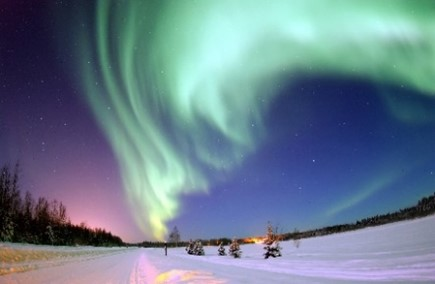
\includegraphics[width=\textwidth]{Instructions/Figs/Regular/Picture1.jpg}
         \caption{}
         \label{fig:a}
     \end{subfigure}
     \hfill
     \begin{subfigure}[b]{0.45\textwidth}
         \centering
         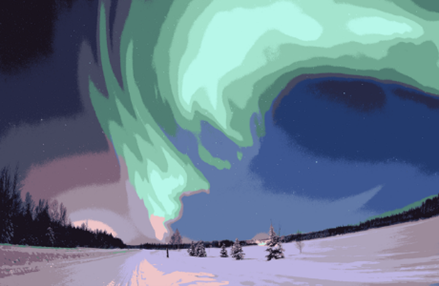
\includegraphics[width=\textwidth]{Instructions/Figs/Regular/Picture2.png}
         \caption{}
         \label{fig:b}
     \end{subfigure}
     \hfill
    \caption{Exemplu de segmentare imagine: (a) imaginea ini\c{t}ial\u{a}, (b) imaginea segmentat\u{a}.}
    \label{fig:exemplu_figura}
\end{figure}
  
\subsection*{Instruc\c{t}iuni pentru Bibliografie}
\begin{itemize}
  \item Referin\c{t}ele bibliografice trebuie plasate la sf\^{a}r\c{s}itul tezei. Este absolut necesar\u{a} referirea la bibliografie \^{i}n textul tezei \c{s}i nu doar listarea referin\c{t}elor bibliografice.
  \item Titlul Bibliografie se scrie cu caractere Times New Roman, bold, de 28pt., la 8 r\^{a}nduri de marginea de sus. Con\c{t}inutul bibliografiei \^{i}ncepe la 2 r\^{a}nduri sub titlu \c{s}i se scrie cu caractere Times New Roman de dimensiune 11pt. O referin\c{t}\u{a} bibliografic\u{a} trebuie s\u{a} con\c{t}in\u{a} toate informa\c{t}iile cu privire la publica\c{t}ie astfel \^{i}nc\^{a}t aceasta s\u{a} fie u\c{s}or identificat\u{a} pentru consultare, exemplu \cite{demarty2014multimodal, duta2017spatio, purica2015multiview}:
\end{itemize}


\noindent
[1] C.-H. Demarty, C. Penet, B. Ionescu, G. Gravier, M. Soleymani, \textit{Multimodal violence detection in Hollywood movies: State-of-the-art and Benchmarking}, Fusion in Computer Vision - Understanding Complex Visual Content, Springer Advances in Computer Vision and Pattern Recognition, pp. 185-208, ISBN: 978-3-319-05695-1, Eds. J. Benois-Pineau, G. Quénot, T. Piatrik, B. Ionescu, 2014.

\noindent
[2] I.C. Duță, B. Ionescu, K. Aizawa, N. Sebe, \textit{Spatio-temporal VLAD Encoding for Human Action Recognition in Videos}, International Conference on Multimedia Modeling - MMM, pp. 365-378, January 4-6, Reykjavík, Iceland, 2017.

\noindent
[3] A.I. Purică, E.G. Mora, B. Pesquet-Popescu, M. Cagnazzo, B. Ionescu, \textit{Multiview plus Depth Video Coding with Temporal Prediction View Synthesis}, IEEE Transactions on Circuits and Systems for Video Technology, 26(2), pp. 360-374, 2016.

\subsection*{Instruc\c{t}iuni \LaTeX}

Instruc\c{t}iunile \LaTeX~se reg\u{a}sesc \^{i}n fi\c{s}ierul README.md.
\thispagestyle{empty}